\documentclass[
    10pt,
    aspectratio=169,
    xcolor={dvipsnames},
    spanish,
    % handout,
    % notes=only,
    % notes,
    ]{beamer}

% BEAMER SETTINGS
\setbeamerfont{section in toc}{size=\normalsize, shape=\bfseries}
\mode<presentation>{
    \usetheme{Antibes}
    \setbeamercovered{transparent}
    \usecolortheme{rose}
    \setbeamertemplate{navigation symbols}{}
    }
\useoutertheme{infolines}
% PACKAGES
% \usepackage[spanish]{babel}  % uncomment for Spanish support
\usepackage{tikz,pgfplots}
\pgfplotsset{compat=1.13}
\usetikzlibrary{calc}
\usepackage{subcaption}
\usepackage{graphicx}
\graphicspath{{figures}}
\usepackage{booktabs}
\usepackage{upgreek}
\usepackage{commath}
\usepackage{amsmath,amsthm,amssymb,mathtools,mathrsfs}
\usepackage{cancel}
\usepackage{fontawesome5}
\usepackage{enumerate}
\usepackage{tensor}
\usepackage[font=footnotesize]{caption}
\usepackage{wasysym}

\usepackage[skins,theorems]{tcolorbox}
\tcbset{
    highlight math style={
        enhanced,
        coltext=black,
        colframe=black,
        colback=lightgray,
        arc=0pt,
        boxrule=.5pt
        }
}

% REFERENCES AND OTHERS
\usepackage{aas_macros}
\usepackage{natbib}
\bibpunct{(}{)}{;}{a}{}{,}

\usepackage{siunitx}
\sisetup{
    range-phrase=\text{--},
    range-units=single,
    separate-uncertainty=true,
    print-unity-mantissa=false
    }
\DeclareSIUnit{\gauss}{G}
\DeclareSIUnit{\jansky}{Jy}
\renewcommand{\figurename}{Fig.}

\usepackage{hyperref}
\hypersetup{
    % bookmarks=true,
    unicode=true,
    pdftoolbar=true,
    pdfmenubar=true,
    pdffitwindow=false,
    pdfstartview={FitH},
    pdftitle={ISI-Free Linear Combination Pulses with Better Performanc},
    pdfauthor={Erik Saez A.},
    pdfcreator={Erik Saez A.},
    pdfnewwindow=true,
    colorlinks=true,
    linkcolor=RoyalBlue,
    citecolor=RoyalBlue,
    urlcolor=RoyalBlue
    }

\title[Auxiliar \#2 - Análisis de Sistemas Dinámicos]{\bfseries Auxiliar \#2 - Análisis de Sistemas Dinámicos}
\subtitle{Función de Transferencia y Respuesta en Frecuencia}
\author[Erik Saez A.]{Erik Saez A.}
\institute[UChile]{Department of Electrical Engineering \\ Universidad de Chile}

\date{\today}

\begin{document}

\begin{frame}
  \titlepage
  \centering
  \faIcon{envelope} \href{mailto:erik.saez@ug.uchile.cl}{erik.saez@ug.uchile.cl} \hspace{.2cm}
\end{frame}

\begin{frame}
  \frametitle{Contenidos}
  \centering
  \begin{columns}
    \begin{column}{0.4\textwidth}
      \tableofcontents
    \end{column}
    \begin{column}{0.5\textwidth}
      \begin{figure}
        \centering
        
\includegraphics[width=\textwidth]{fcfm_die}
        \caption{Facultad de Ciencias Físicas y Matemáticas, Universidad de Chile.}
      \end{figure}
    \end{column}
  \end{columns}  
\end{frame}
%%%%%%%%%%%%%%%%%%%%%%%%%%%%%%%%%%%%%%%%%%

\section{Resumen de Conceptos}

\begin{frame}{Clasificación de Sistemas Dinámicos}
\begin{block}{Criterios de Clasificación}
  Los criterios de clasificación de un sistema son maneras de \textbf{organizar y categorizar} los sistemas dinámicos en función de sus características y comportamientos.
  \begin{table}[h]
    \centering
    \begin{tabular}{|l|l|}
    \hline
    \textbf{Punto de vista} & \textbf{Clasificación} \\
    \hline
    Origen & Naturales - Artificiales \\
    \hline
    Naturaleza & Determinísticos - Aleatorios \\
    \hline
    Número de variables & Monovariables - Multivariables \\
    \hline
    Continuidad de variables & Variables discretas - continuas \\
    \hline
    Comportamiento espacial & Variables concentradas - distribuidas \\
    \hline
    Comportamiento temporal & Variable - Invariante \\
    \hline
    Linealidad de variables & Lineales - No lineales \\
    \hline
    Realizabilidad & Causales - Anticipativos \\
    \hline
    \end{tabular}
  \end{table}
\end{block}
\end{frame}

%%%%%%%%%%%%%%%%%%%%%%%%
%%%%%%%%%%%%%%%%%%%%%%%%
\begin{frame}{Análisis en Frecuencia}
\begin{block}{Introducción}
  \footnotesize
  Muchas veces el análisis de un sistema determinado se facilita si se realiza en función de su frecuencia, en vez del tiempo. Para esto existen distintas herramientas, tanto analíticas como computacionales, que sirven para distintos tipos de sistemas.
\end{block}

\begin{columns}
  \begin{column}{0.48\textwidth}
    \begin{block}{Transformada de Laplace}
      \footnotesize
      Se definen la transformada de Laplace unilateral y bilateral como:
      
      \textbf{Unilateral:} 
      $$\mathcal{L}\{f(t)\} = F(s) := \int_0^{\infty} f(t)e^{-st}dt$$
      
      \textbf{Bilateral:} 
      $$\mathcal{L}\{f(t)\} = F(s) := \int_{-\infty}^{\infty} f(t)e^{-st}dt$$
      
      donde $s = \sigma + j\omega$ es la "frecuencia compleja". Generalmente, las funciones resultantes de una transformada de Laplace se escriben con mayúsculas.
    \end{block}
  \end{column}
  
  \begin{column}{0.48\textwidth}
    \begin{block}{Propiedades Importantes}
      \footnotesize
      Esta transformada cumple con tres propiedades importantes:
      \begin{itemize}
        \item \textbf{Linealidad:} 
        $$\mathcal{L}\{af(t) + bg(t)\} = aF(s) + bG(s)$$
        \item \textbf{Desplazamiento:} 
        $$\mathcal{L}\{e^{at}f(t)\} = F(s-a)$$
        $$\mathcal{L}\{f(t-a)\} = e^{-as}F(s)$$
      \end{itemize}
    \end{block}
  \end{column}
\end{columns}
\end{frame}

%%%%%%%%%%%%%%%%%%%%%%%%
\begin{frame}{Análisis en Frecuencia}
\begin{columns}
  \begin{column}{0.55\textwidth}
    \begin{block}{Definición}
      \footnotesize
      Una de las utilidades de la transformada de Laplace es que tiene una inversa:
      $$\mathcal{L}^{-1}\{F(s)\} = f(t) := \frac{1}{2\pi j} \int_{\sigma-j\infty}^{\sigma+j\infty} F(s)e^{st}ds$$
    \end{block}
    
    \begin{block}{Antitransformadas Típicas}
      \footnotesize
      \begin{itemize}
        \item $\mathcal{L}^{-1}\left\{\frac{1}{s}\right\} = 1$ \qquad $\mathcal{L}^{-1}\left\{\frac{1}{s^2}\right\} = t$
        \item $\mathcal{L}^{-1}\left\{\frac{1}{s+a}\right\} = e^{-at} \qquad \mathcal{L}^{-1}\left\{\frac{1}{s^2+a^2}\right\} = \frac{\sin(at)}{a}$
        \item $\mathcal{L}^{-1}\left\{\frac{s}{s^2+a^2}\right\} = \cos(at) \qquad \mathcal{L}^{-1}\left\{\frac{n!}{s^{n+1}}\right\} = t^n$
      \end{itemize}
    \end{block}
  \end{column}
  
  \begin{column}{0.4\textwidth}
    \begin{block}{Transformadas Básicas}
      \footnotesize
      \begin{itemize}
        \item $\mathcal{L}\{t^n f(t)\} = (-1)^n \frac{d^n}{ds^n} F(s)$
        \item $\mathcal{L}\{\delta(t)\} = 1$
        \item $\mathcal{L}\{(f * g)(t)\} = F(s)G(s)$
        \item $\mathcal{L}\{f^n(t)\} = s^n F(s) - s^{n-1}F(0) - s^{n-2}F'(0) - \cdots$
        \item $\mathcal{L}\left\{\int_0^t f(\tau)d\tau\right\} = \frac{F(s)}{s}$
        \item $F(s) = \frac{1}{1-e^{-sT}} \int_0^T f(s)e^{-st}dt$ si $f(t)$ $T$ periódica
      \end{itemize}
    \end{block}
  \end{column}
\end{columns}
\end{frame}

%%%%%%%%%%%%%%%%%%%%%%%%
\begin{frame}{Polos y Función de Transferencia}
\begin{columns}
  \begin{column}{0.48\textwidth}
    \begin{block}{Función de Transferencia}
      \footnotesize
      Para sistemas lineales e invariantes en el tiempo, cuando se realiza un análisis en el dominio de Laplace es posible definir:
      $$H(s) = \frac{Y(s)}{U(s)}$$
      donde $Y(s)$ y $U(s)$ son las transformadas de Laplace de la salida y la entrada, respectivamente.
      
      Esta función caracteriza completamente el comportamiento dinámico del sistema.
    \end{block}
    
    \begin{block}{Descomposición en Fracciones Parciales}
      \footnotesize
      \textbf{Polos simples:} Para $H(s) = \frac{N(s)}{(s+a)D(s)}$:
      $$H(s) = \frac{A}{s+a} + \frac{B(s)}{D(s)}$$
      donde $A = H(s)(s+a)|_{s=-a}$
    \end{block}
  \end{column}
  
  \begin{column}{0.48\textwidth}
    \begin{block}{Tipos de Polos}
      \footnotesize
      \begin{itemize}
        \item \textbf{Polos reales negativos}: $s = -a$ (con $a > 0$)
        \\$\rightarrow$ Respuesta exponencial decreciente $e^{-at}$
        \item \textbf{Polos complejos conjugados}: $s = -\sigma \pm j\omega$
        \\$\rightarrow$ Respuesta oscilatoria amortiguada
        \item \textbf{Polos en el origen}: $s = 0$
        \\$\rightarrow$ Respuesta escalón o rampa
        \item \textbf{Polos múltiples}: Raíces repetidas
        \\$\rightarrow$ Términos con $t^n e^{-at}$
      \end{itemize}
    \end{block}
    
    \begin{alertblock}{Estabilidad}
      \footnotesize
      Un sistema es estable si todos sus polos tienen parte real negativa (están en el semiplano izquierdo del plano $s$).
    \end{alertblock}
  \end{column}
\end{columns}
\end{frame}



%%%%%%%%%%%%%%%%%%%%%%%%
\section{Pregunta 1}
\begin{frame}{Pregunta \#1}
\begin{columns}
  \begin{column}{0.6\textwidth}
    \begin{block}{Enunciado Pregunta \#1}
    \footnotesize
    Considere el siguiente circuito eléctrico, donde \(\alpha(t)i_2(t)\) corresponde al valor de la resistencia eléctrica de un potenciómetro, cuyo valor depende tanto de \(\alpha(t)\) como de la corriente que circula por el condensador, y \(v_{out}(t)\) (voltaje en el condensador) se mide con un voltímetro.
    
    \begin{enumerate}
        \item Establezca claramente el listado de hipótesis simplificatorias que permitan
        establecer un modelo matemático válido para este sistema. Indique las condiciones de borde y/o
        iniciales necesarias.
        \item Formule un modelo para el sistema en ecuaciones de estado.
        \item Caracterice completamente el modelo utilizando todos los puntos de vista descritos en clases.
        Clasifique todas las variables del sistema.
        \item Encuentre estado(s) cero, estado(s) de equilibrio y el estado tierra (de existir).
        \item Linealice el sistema en torno al (los) estado(s) de equilibrio encontrados.
    \end{enumerate}
    \end{block}
  \end{column}
  
  \begin{column}{0.4\textwidth}
    \begin{figure}[ht]
        \centering
        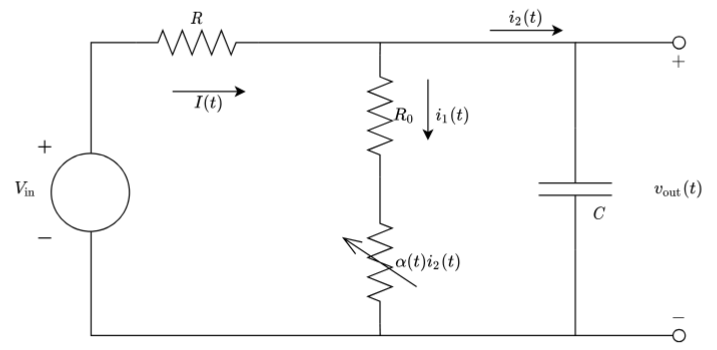
\includegraphics[width=\textwidth]{Auxiliar_2_1.png}
    \end{figure}
  \end{column}
\end{columns}
\end{frame}
%%%%%%%%%%%%%%%%%%%%%%
\section{Pregunta 2}
\begin{frame}{Pregunta \#2}
  \begin{block}{Enunciado Pregunta \#2}
   Considere el sistema linealizado del auxiliar anterior, modelado por la siguiente ecuación diferencial:
    \begin{equation}
        \ddot{\theta}(t) = \frac{g}{l} \theta(t) + \frac{1}{l} u(t)
    \end{equation}

    \begin{enumerate}
        \item Descomponer la salida como la suma de la respuesta a condiciones iniciales nulas y la respuesta a entrada nula en el dominio de Laplace.
        \item Obtener la función de transferencia del sistema y encontrar la respuesta al impulso con condiciones iniciales nulas en el dominio del tiempo.
        \item Obtener la respuesta a entrada nula en el dominio del tiempo, y expresar la respuesta para una entrada y condiciones iniciales arbitrarias.
        \item Encuentre la salida cuando la entrada es un escalón unitario
    \end{enumerate}
  \end{block}
\end{frame}

\end{document}
